\chapter{はじめに}
\thispagestyle{myheadings}

\section{背景}
\label{sec:background}

近年,人の歌声や喋り声をコンピュータ上で再現する音声合成ソフトウェアは楽曲制作やアナウンスなどに広く利用されており,その普及と同時に音声合成ソフトウェアの数も増加している.
合成音声ソフトウェアの多くは合成音声ライブラリを切り替えて合成される声の種類を変更でき,ユーザが利用できる声の種類はソフトウェアの数以上に存在する.
加えて,いくつかのソフトでは個人のユーザが自分の声からライブラリを作成して第三者に配布でき,そのようなソフトではライブラリ数は非常に多くなる.
例えば,喋り声を対象とした合成音声ソフトCOEIROINKではユーザの作成した音声合成モデルが350キャラクタ分以上配布されている\cite{mycoeiroink}ほか,歌声を対象とした合成音声ソフトUTAUでは同ソフト上で使用できるUTAU音源ライブラリが7000キャラクタ分以上存在する\cite{vdbutau}.
このように,合成音声ソフトの利用者は使える声に対し非常に多くの選択肢を持っている.

合成音声を利用するシーンにおいて,声の持つイメージや印象は声を選ぶ上で考慮すべき要素である.
例えば,重要な情報をアナウンスする際に滑舌の悪い声を使うと情報が正しく伝達できない可能性があり,可愛らしく軽快な楽曲に対して力強い声を使用すると聞き手に違和感を与える恐れがある.
用途に合った声質を持つライブラリの採択は,情報を伝える効果や楽曲の表現力の向上に寄与する.
しかし,現状声の持つ印象を知るには実際に聴いてみるのが最も有力な手段であり,数多あるライブラリの生み出す声を十分な数聴き比べ適切な声を採択するには多大な手間と時間を要する.
その結果として,ユーザがライブラリを選ぶ際にその多くが普段の生活の中で聞いた経験のある声や,知っているキャラクターの声を選択していると考えられ,ユーザ全体の中で使われる声には大きな偏りが生じている.
万に近い数存在するライブラリのうち実際にユーザに用いられる声は一握りであり,ほとんどのライブラリはユーザに用いられず埋もれてしまう.

\section{研究目的とアプローチ}
本研究の目的は,多くの合成音声ライブラリの中から,ユーザの用途に合った声・ユーザのイメージする声に近い声を探索する効率的な手法の,実際にユーザが使用可能な形式での提案である.
このような手法が実現できれば,ユーザは声質に対する自身の要求を入力するだけで,膨大な数の合成音声ライブラリの中から要求に合った声を持つライブラリを効率的に採択できるようになる.
これにより,ユーザは従来のように実際に多くの声を聴き比べる必要がなくなり,声の選択にかかる労力を大幅に削減できる.
また,純粋にライブラリの持つ声質のみでの探索はこれまで埋もれていた多様な声質を持つライブラリの発掘にもつながり,合成音声ライブラリの制作者とユーザの双方への利益が期待できる.

本研究では,ライブラリごとの声に対する印象を数値化する機械学習モデルを構築し,それを用いてユーザの求める声に近いUTAU音源ライブラリを探索するWebサービス「声色見本帳」を提案する.
サービスの概要を図\ref{fig:fig1}に示す.
サービスを利用するユーザはまず,用途に合った声や自分の求める声をイメージし,サービスで用いる7つの評価軸に基づいてその声に対する評価スコアを数値化する.
評価スコアは評価軸ごとに声に対する印象を1〜7の数値で表すもので,例えば「性別感」という軸では,スコアの高低を男性らしい声・女性らしい声に対応させるなど,スコアと声の関係を理解しやすい評価軸を用いている.
例えば女性らしい声を求める場合,「性別感」軸のスコアを2など低い数値に設定する.
求める声のイメージを評価スコアとして数値化し入力すると,サービスは登録されているライブラリのスコアと入力されたスコアを比較し,声の近いライブラリを複数提案する.
ユーザは求める声に似ていると提案されたいくつかのライブラリを聴き比べ,自分の求める声に近いライブラリを少ない手間で探索できる.

\begin{figure}[htb]
  \centering
  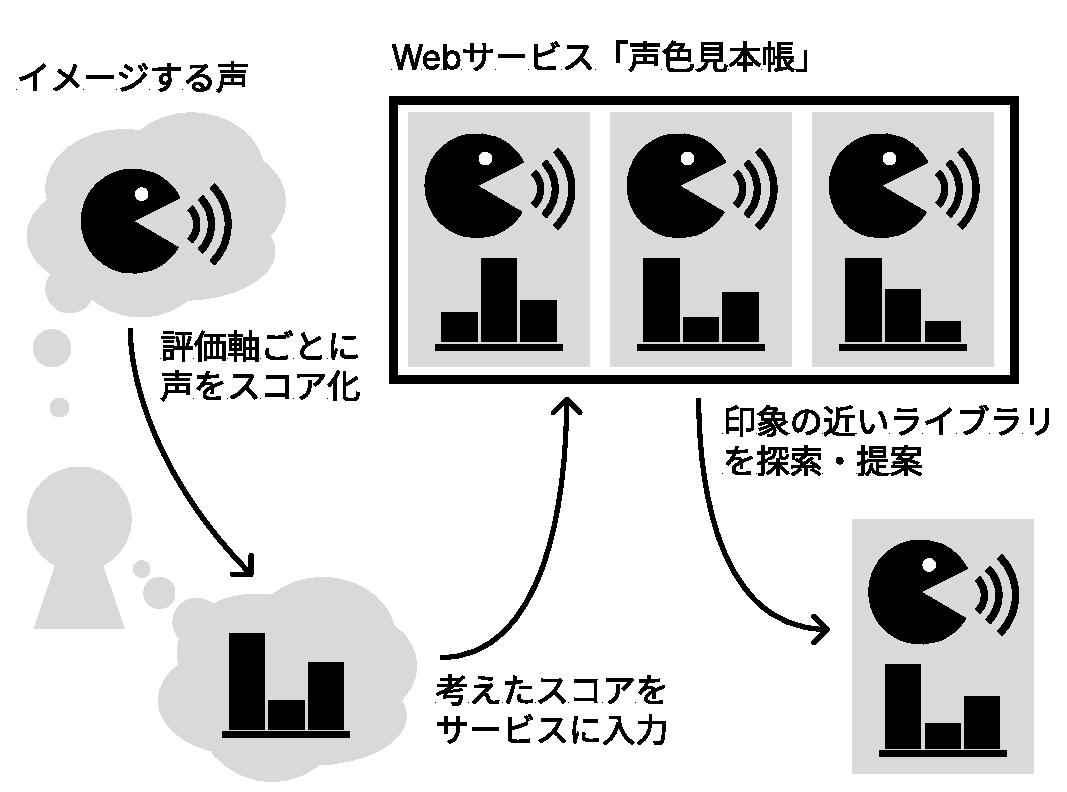
\includegraphics[width=0.9\linewidth]{fig/fig1.pdf}
  \caption{提案するサービス「声色見本帳」の概要}
  \label{fig:fig1}
\end{figure}

提案するサービスでは,探索対象として登録されたライブラリごとの評価スコアを事前に設定する必要がある.
声に対する印象を数値化するための評価スコアを得るには,アンケート調査の実施が方法として考えられる.
しかし,アンケート調査には多くの時間と労力が必要であり,多くのライブラリに対してのアンケート調査は困難である.
そこで,本研究では事前にいくつかのライブラリに対してアンケート調査を行ない,そのデータを用いてライブラリごとの声に対する評価スコアを推定する機械学習モデルを構築する.
機械学習モデルを用いた評価スコアの推定の概要を図\ref{fig:fig2}に示す.
構築したモデルを用いれば,アンケート調査を行なっていないライブラリに対しても評価スコアを機械的に,一定の精度を持って付与できる.
機械学習モデルを用い,より多くのライブラリを探索対象として登録できるほか,今後新たに公開されるライブラリに対しても効率的に評価スコアを付与できる.

\begin{figure}[htb]
  \centering
  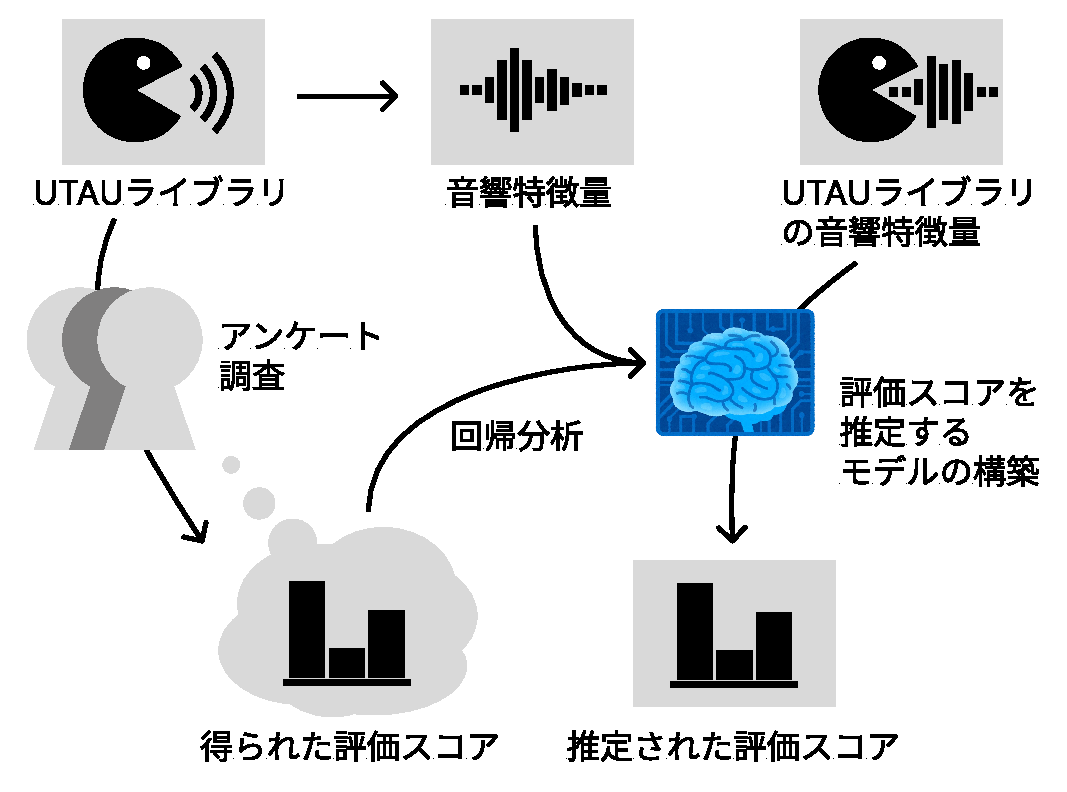
\includegraphics[width=0.9\linewidth]{fig/fig2.pdf}
  \caption{評価スコアを推定するモデルの構築イメージ}
  \label{fig:fig2}
\end{figure}

本サービスではUTAU音源ライブラリを探索対象として選定した.
UTAU音源ライブラリは,無償で公開されている歌唱用音声合成ソフトウェアであるUTAU,およびその互換ソフトウェア上で使用できるライブラリであり,このライブラリを切り替えると実際に合成される音声を変更できる.
UTAU音源ライブラリは\ref{sec:background}節でも触れたように数が特に多く,そのほとんどを無料で利用できるため,多様な声質を持つライブラリを探索するメリットが大きいと考えられるためである.
また,UTAU音源ライブラリには声質に関する調査を行なったアンケートデータが既存するため,機械学習モデルの構築に用いるデータセットの作成が容易である点も選定の理由である.
なお,UTAU音源ライブラリを利用し構築したモデルでも,他の合成音声ソフトの音源ライブラリに対して適用が可能であり,将来的にUTAU音源ライブラリ以外のライブラリに対しても探索できるようサービスを拡張できる.

\section{本論文の構成}
本論文の構成は以下の通りである.
第2章では,関連研究について述べる.
第3章では,ライブラリから評価スコアを推定する機械学習モデルの構築と,構築したモデルの推論精度に対する評価実験について述べる.
第4章では,提案するサービス「声色見本帳」の設計と実装について述べる.
最後に第5章として本論文のまとめと今後の課題について述べる.

% Local Variables:
% mode: japanese-LaTeX
% TeX-master: "root"
% End:
